\documentclass[pdf,slideColor,fyma]{beamer}

\usepackage{ucs}
\usepackage[utf8]{inputenc}
\usepackage[czech,english]{babel}

\usepackage{color}
\usepackage{graphics}
\usepackage{picture}
\usepackage{amsfonts}
\usepackage{float}
\usepackage{wrapfig}

\title{Jóga}
\author{Jan Ondruch \\ {\footnotesize xondru14@fit.vutbr.cz}}
\institute{Fakulta informačních technologií \\ Vysoké učení technické v~Brně}
\date{\today}

\begin{document}

\begin{frame}
	\titlepage
\end{frame}
%%%%%%%%%%%%%%%%%%%%%%%%%%%%%%%
\begin{frame}{Co je to Jóga?}
	\begin{center}
    Jóga je označení pro fyzickou, mentální a spirituální disciplínu, která má kořeny ve staré Indii.
  	\end{center}  
\end{frame}
%%%%%%%%%%%%%%%%%%%%%%%%%%%%%%%
\begin{frame}{Cíle jógy}
	Konečný cíl jógy je dosáhnutí {\itshape moksha} (osvobození). Existují však různorodé definice, čeho {\itshape moksha} vlastně dosahuhje.
	\medskip
	\begin{figure}[H]
  		\centering
		\scalebox{0.33}{
\includegraphics{joga1.eps}}
	\end{figure}	  
\end{frame}
%%%%%%%%%%%%%%%%%%%%%%%%%%%%%%%
\begin{frame}{Širší význam slova  {\itshape jóga}}
	Dle např. \textbf{Jakobsena}, "Jóga má 5 hlavních významů."
	\medskip
	\begin{enumerate}
		\item Jóga je disciplinovaná metoda pro dosažení cíle
		\item Jóga jako soubor praktik pro kontrolu těla a~mysli
		\item Jóga jako jméno školy nebo filosofického systému {\itshape darsána}
		\item Jóga ve spojení s~jinými slovy, jako např. {\itshape hatha-}, které se odkazují na tradiční speciální techniky jógy
		\item Jóga jako cíl praktikování jógy
	\end{enumerate}
\end{frame}
%%%%%%%%%%%%%%%%%%%%%%%%%%%%%%%
\begin{frame}{Školy}
	Základní školy jógy rozvíjející se již po staletí v~náboženských a~filozofických systémech.
	\medskip
	\begin{wrapfigure}{r}{0.5\textwidth}
	\begin{figure}
  		\begin{center}
    			\scalebox{0.25}{
\includegraphics{joga2.eps}}
  		\end{center}
	\end{figure}
	\end{wrapfigure}
	\begin{itemize}
		\item Buddhismus
		\item Hinduismus
		\item Jainismus
		\item Tantra
	\end{itemize}
\end{frame}
%%%%%%%%%%%%%%%%%%%%%%%%%%%%%%%
\begin{frame}{Moderní jóga}
	Je rozšířená po celém světě díky svým befefitům pro lidské tělo.
	\medskip
	\begin{itemize}
		\item Zlepšuje flexibilitu
		\item Detoxikuje tělo
		\item Posiluje svaly
		\item Promazává klouby, vazy, šlachy
		\item Zbavuje stresu a~poskytuje uvolnění
		\item \dots
	\end{itemize}
\end{frame}
%%%%%%%%%%%%%%%%%%%%%%%%%%%%%%%
\begin{frame}{Začít můžete kdykoliv!}
	\begin{center}
    		Pokud nejste spokojeni se svým zdravotním stavem, právě jóga pro Vás může být tou správnou volbou. \\
    		\bigskip
    		20 minut 3--4x týdně {\large{bohatě stačí}}.
    		\begin{center}
    			\scalebox{0.33}{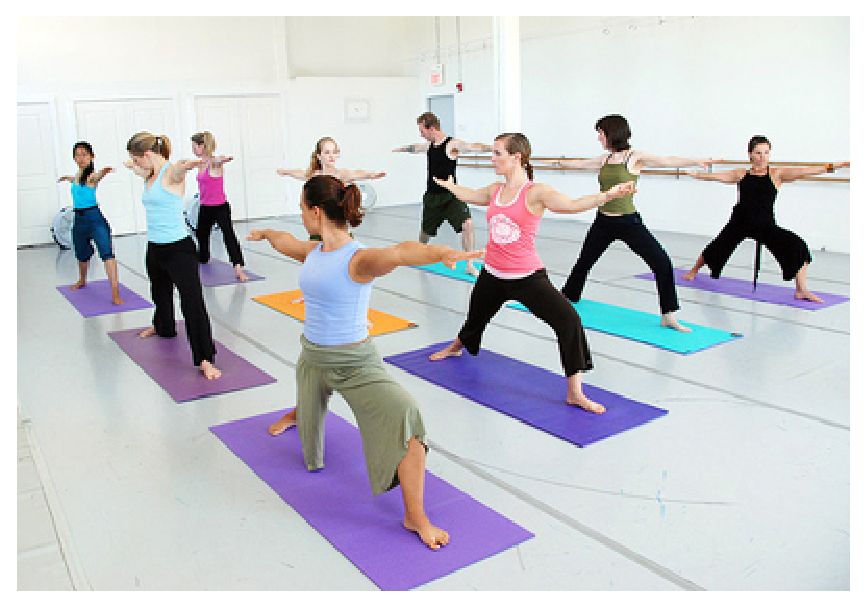
\includegraphics{joga4.eps}}
  		\end{center}   
  	\end{center} 
\end{frame}
%%%%%%%%%%%%%%%%%%%%%%%%%%%%%%%
\begin{frame}{Konec}
	\begin{center}
		Děkuji za pozornost!
		\medskip
		\begin{center}
    			\scalebox{0.25}{
\includegraphics{joga3.eps}}
  		\end{center}
	\end{center}
\end{frame}

\end{document}